
\documentclass[10pt,reprint,aps,onecolumn,nofootinbib]{revtex4-2}
% ====== minimal packages ======
\usepackage{amsmath,amssymb,amsfonts}
\usepackage{bm}
\usepackage{physics}
\usepackage{microtype}
\usepackage{tcolorbox}
\usepackage{mathtools}

% load hyperref *after* natbib
\usepackage[colorlinks=true,linkcolor=blue,citecolor=blue,urlcolor=blue]{hyperref}
\usepackage[utf8]{inputenc}
\usepackage[T1]{fontenc}
\usepackage[margin=2.2cm]{geometry}



% ==== Packages ====
\usepackage{lmodern}
\usepackage{booktabs}
\usepackage[caption=false]{subfig}
\usepackage{tikz}
\usetikzlibrary{arrows.meta,positioning,calc,fit,decorations.pathmorphing}
\pdfstringdefDisableCommands{%
    \def\boldsymbol#1{#1}%
    \def\mathcal#1{#1}%
    \def\!{}%
    \def\swirlarrow{}% if you use that macro in titles
}

% swirl arrows (context-aware)
\DeclareRobustCommand{\swirlarrow}{%
    \mathchoice{\mkern-2mu\scriptstyle\boldsymbol{\circlearrowleft}}%
    {\mkern-2mu\scriptstyle\boldsymbol{\circlearrowleft}}%
    {\mkern-2mu\scriptscriptstyle\boldsymbol{\circlearrowleft}}%
    {\mkern-2mu\scriptscriptstyle\boldsymbol{\circlearrowleft}}%
}
\newcommand{\paperversion}{\textbf{v0.0.1}}
\newcommand{\papertitle}{Rotating--Frame Unification in the SST Canon: From Swirl Density to Swirl--EMF, and a Canonical Derivation of the Coupling G_swirl}
\newcommand{\paperdoi}{10.5281/zenodo.17203813}


\usepackage{graphicx}
\begin{document}

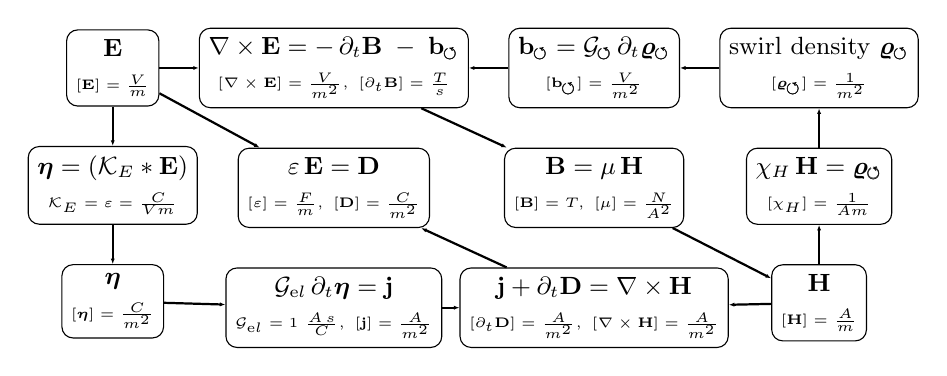
\begin{tikzpicture}[
    node distance=0.5 and 0.5,
    every node/.style={draw, rounded corners, align=center, minimum height=2},
    arrow/.style={-{Latex[length=2]}, thick},
    garrow/.style={-{Latex[length=2]}, thick, dashed}
]
% ---------------- TOP LAYER ----------------
% ---------------- center left curl (Faraday) ----------------
\node(Faraday)
{
    \small$\nabla \times \mathbf{E} = -\,\partial_t \mathbf{B} \;-\; \mathbf{b}_{\swirlarrow}$\\
    \tiny $[\nabla\times\mathbf E]=\tfrac{V}{m^{2}},\ [\partial_t\mathbf B]=\tfrac{T}{s}$};

% ---------------- left: field E ----------------
\node[left=of Faraday]  (E)
{
    \small$\mathbf{E}$\\
    \tiny $[\mathbf E]=\tfrac{V}{m}$
};

% ---------------- center right:  b ----------------
\node[right=of Faraday] (b)
{
    \small $\mathbf b_{\swirlarrow}=\mathcal G_{\swirlarrow}\,\partial_t\bm{\varrho}_{\swirlarrow}$\\
    \tiny  $[\mathbf b_{\swirlarrow}]=\tfrac{V}{m^{2}}$};

% ---------------- right: swirl density rho ----------------
\node[right=of b] (rho)
{
    \small swirl density $\bm{\varrho}_{\swirlarrow}$\\
    \tiny  $[\bm{\varrho}_{\swirlarrow}]=\tfrac{1}{m^{2}}$};


% ---------------- Middle layer ----------------
% ---------------- left: conduction accumulation ----------------
\node[below=of E] (Eta)
{
    \small $\bm{\eta} = (\mathcal K_E * \mathbf E)$\\
    \tiny  $\mathcal K_E = \varepsilon = \frac{C}{Vm}$};

% ---------------- center left right D, B ----------------
\node[below=of Faraday] (D)
{
    \small $\varepsilon\,\mathbf{E} = \mathbf{D}$\\
    \tiny  $[\varepsilon]=\tfrac{F}{m},\ [\mathbf D]=\tfrac{C}{m^{2}}$};

\node[below=of b] (B)
{
    \small $\mathbf{B}=\mu\,\mathbf{H}$\\
    \tiny  $[\mathbf B]=T,\ [\mu]=\tfrac{N}{A^{2}}$};

% ---------------- right: susceptibility ----------------
\node[below=of rho] (C)
{
    \small $\chi_H\,\mathbf{H} = \bm{\varrho}_{\swirlarrow}$\\
    \tiny  $[\chi_H]=\tfrac{1}{Am}$};

% ---------------- Bottom layer ----------------
% --- bottom-left areal density (now the visible card) ---
\node[below=of Eta] (EtaBottom)
{
    \small $\bm{\eta}$\\
    \tiny  $[\bm{\eta}]=\tfrac{C}{m^{2}}$};

% --- flying source card below (derivative step) ---
\node[below=of D] (Jsrc)
{
    \small $\mathcal G_{\textrm el}\, \partial_t \bm{\eta} = \mathbf{j}$\\
    \tiny  $\mathcal G_{\textrm el}=1~\tfrac{A \, s}{C},\ [\mathbf j]=\tfrac{A}{m^{2}}$};

% ---------------- Ampère curl ----------------
\node[below=of  B] (Ampere)
{
    \small $\mathbf{j} + \partial_t \mathbf{D} = \nabla \times \mathbf{H}$\\
    \tiny  $[\partial_t\mathbf D]=\tfrac{A}{m^{2}},\ [\nabla\times\mathbf H]=\tfrac{A}{m^{2}}$};

% ---------------- right bottom: H ----------------
\node[below=of C] (H)
{
    \small $\mathbf{H}$\\
    \tiny  $[\mathbf H]=\tfrac{A}{m}$};


% ---------------- arrows (same geometry as your framework) ----------------
\draw[arrow] (E) -- (D);
\draw[arrow] (C) -- (rho);
\draw[arrow] (H) -- (Ampere);
\draw[arrow] (E) -- (Faraday);
\draw[arrow] (Faraday) -- (B);
\draw[arrow] (Ampere) -- (D);
\draw[arrow] (B) -- (H);
\draw[arrow] (H) -- (C);

% --- replaced Ohm path by the mirrored left ladder ---
\draw[arrow] (E) -- (Eta);          % kernel stage
\draw[arrow] (Eta) -- (EtaBottom);  % field -> areal density (visible bottom card)
\draw[arrow] (EtaBottom) -- (Jsrc); % derivative to source (flying)
\draw[arrow] (Jsrc) -- (Ampere);    % feeds Ampère

% --- long-range mediation on the right stays ---
\draw[arrow] (rho) --  (b);
\draw[arrow] (b) -- (Faraday);

\end{tikzpicture}

\\
\scriptsize $[\nabla\times\mathbf E]=\tfrac{V}{m^{2}}$,\\
$[\partial_t\mathbf B]=\tfrac{T}{s}$
\\ \scriptsize $[\mathbf E]=\tfrac{V}{m}$
\\ $[\bm{\varrho}_{\swirlarrow}]=\tfrac{1}{m^{2}}$
\\
\scriptsize $[\mathbf b_{\swirlarrow}]=\tfrac{V}{m^{2}}$
\\
\scriptsize $[\chi_H]=\tfrac{1}{Am}$
\\
$\mathcal K_E = \varepsilon = \frac{C}{Vm}$
\\
\scriptsize $[\varepsilon]=\tfrac{F}{m}$\\
$[\mathbf D]=\tfrac{C}{m^{2}}$
\\
\scriptsize $[\mathbf B]=T $\\
$[\mu]=\tfrac{N}{A^{2}}$
\\
\scriptsize $[\bm{\eta}]=\tfrac{C}{m^{2}}$
\\
\scriptsize $\mathcal G_{\textrm el}=1~\tfrac{A \, s}{C}$,\\
$[\mathbf j]=\tfrac{A}{m^{2}}$
\\
\scriptsize $[\partial_t\mathbf D]=\tfrac{A}{m^{2}}$\\
$[\nabla\times\mathbf H]=\tfrac{A}{m^{2}}$
\\ \scriptsize $[\mathbf H]=\tfrac{A}{m}$




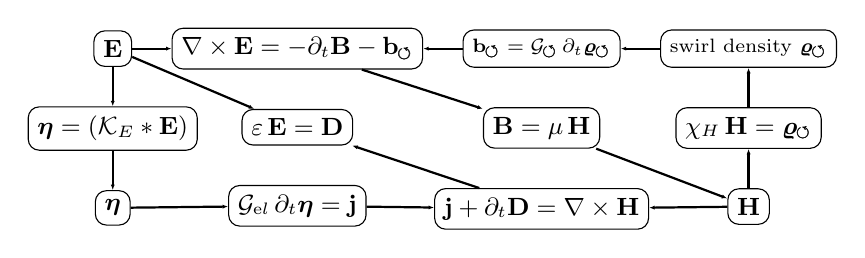
\begin{tikzpicture}[
    node distance=0.5 and 0.5,
    every node/.style={draw, rounded corners, align=center, minimum height=2, font=\small},
    arrow/.style={-{Latex[length=2]}, thick},
    garrow/.style={-{Latex[length=2]}, thick, dashed}
]
% ---------------- center curl (Faraday) ----------------
\node(Faraday)
{$\nabla \times \mathbf{E} = -\partial_t \mathbf{B} - \mathbf{b}_{\swirlarrow}$};

% ---------------- left: field E ----------------
\node[left=of Faraday]  (E)
{$\mathbf{E}$};

\node[right=of Faraday] (b)
{\scriptsize $\mathbf b_{\swirlarrow}=\mathcal G_{\swirlarrow}\,\partial_t\bm{\varrho}_{\swirlarrow}$};
% ---------------- right: swirl density rho ----------------
\node[right=of b] (rho)
{\scriptsize swirl density $\bm{\varrho}_{\swirlarrow}$};

% ---------------- right middle: susceptibility ----------------
\node[below=of rho] (C)
{$\chi_H\,\mathbf{H} = \bm{\varrho}_{\swirlarrow}$};

% ---------------- left middle: conduction accumulation ----------------
\node[below=of E] (Eta)
{$\bm{\eta} = (\mathcal K_E * \mathbf E)$};

% ---------------- constitutive B,D ----------------
\node[below=of Faraday] (D)
{$\varepsilon\,\mathbf{E} = \mathbf{D}$};

\node[below=of b] (B)
{$\mathbf{B}=\mu\,\mathbf{H}$};

% --- bottom-left areal density (now the visible card) ---
\node[below=of Eta] (EtaBottom)
{$\bm{\eta}$};

% --- flying source card below (derivative step) ---
\node[below=of D] (Jsrc)
{$\mathcal G_{\textrm el}\, \partial_t \bm{\eta} = \mathbf{j}$};

% ---------------- Ampère curl ----------------
\node[below=of B] (Ampere)
{$\mathbf{j} + \partial_t \mathbf{D} = \nabla \times \mathbf{H}$};

% ---------------- right bottom: H ----------------
\node[below=of C] (H)
{$\mathbf{H}$};


% ---------------- arrows (same geometry as your framework) ----------------
\draw[arrow] (E) -- (D);
\draw[arrow] (C) -- (rho);
%\draw[arrow] (rho) -- (Faraday);
%\draw[arrow] (EtaBottom) -- (Ampere);
\draw[arrow] (H) -- (Ampere);
\draw[arrow] (E) -- (Faraday);
\draw[arrow] (Faraday) -- (B);
\draw[arrow] (Ampere) -- (D);
\draw[arrow] (B) -- (H);
\draw[arrow] (H) -- (C);

% --- replaced Ohm path by the mirrored left ladder ---
\draw[arrow] (E) -- (Eta);          % kernel stage
\draw[arrow] (Eta) -- (EtaBottom);  % field -> areal density (visible bottom card)
\draw[arrow] (EtaBottom) -- (Jsrc); % derivative to source (flying)
\draw[arrow] (Jsrc) -- (Ampere);    % feeds Ampère

% --- long-range mediation on the right stays ---
\draw[arrow] (rho) --  (b);
\draw[arrow] (b) -- (Faraday);


\end{tikzpicture}

\end{document}